% replace all text with your own text.
% in this template few examples are mention
\chapter{Methodology}
\label{ch:method} % Label for method chapter


\section{Data Collection}
Initially, the goal is to collect a large variety of information from many sources in order to have a thorough knowledge of the variables that lead to lung disease epidemics. Having access to both past and present information is made easier by partnerships with research groups, health departments, and healthcare organizations. Additionally, social media and internet-based sources of information complement traditional data streams, adding neighbourhood medical trends and public views of symptoms related to breathing to the dataset. A lung disease dataset is chosen from an online source Kaggle which contains the image of chest X-rays of 4 lung-related diseases. The model's input dataset is composed of multiple lung X-rays that have been gathered over time and labelled with four distinct breathing conditions. 
\subsection{Data Analysis}
\label{subsec:se_chpters}
A comprehensive analysis is performed on the gathered data to identify trends, patterns, and relationships related to lung disease epidemics. To learn more about the features of the dataset, initial investigation methods include data visualization, relationship matrices, and general statistics. Then, correlations between putative risk variables and the incidence of lung disease outbreaks are found using sophisticated statistical techniques including regression modelling and period analysis. Machine learning methods are used to find complicated relationships in the information, such as support vector machines and decision tree techniques. Preferences for choosing a model include understanding, adaptability, and reliability across various demographics and geographical areas. The accuracy and significance of data are improved for predictive modelling by data preparation. Enhancing the efficiency of models entails implementing features in addition to maintenance, normalizing, and assigning values that are not present. Overfitting hazards and computational difficulty are minimized through selected features and the reduction of dimensionality algorithms. Different test datasets are used in validation processes like bootstrapping to evaluate the efficiency and adaptability of the model. Compatibility with clinical standards and best practices is ensured by working alongside subject specialists.


\subsection{Data Processing}
Python simplifies interacting with data easier for users by providing a large number of built-in libraries for data processing and visualization. By highlighting trends and correlations, graphical representations of data, such as graphs and charts, make it easier to analyse and examine the data. Matplotlib and Seaborn are two popular Python libraries for data visualization that are available for usage in this context. These libraries include a variety of graphs that exhibit data in diverse ways, such as line plots, bar plots, and histograms. Density charts, for example, are useful for showing the shape of data and for calculating the probability density function and ongoing dataset allocation. By visualising data set descriptions and statistical distributions, box plots, on the other hand, are a useful tool for identifying possible outliers. 
\begin{figure}[ht]
    \centering
    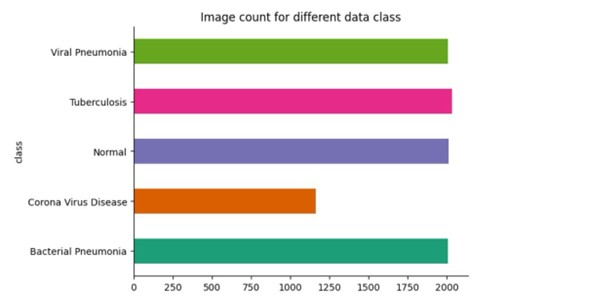
\includegraphics[scale=0.3]{figures/graph.jpg}
    \caption{Example figure in \LaTeX.}
    \label{fig:chart_a}
\end{figure}

Further processing the data, the dataset is split into 3 parts. 60 percent of the data is divided into training , 20 percent data is divided into validation and the remaining 20 percent of the data is divided into testing parts. This distributed dataset is passed on as input to train the models in a much more efficient and uniform manner. By splitting up the data set into training and testing sections, it is possible to train the model on the first one and assess its performance on the remaining part while the validation part will ensure the model’s accuracy on the trained data.In order for the model to train efficiently and produce precise predictions, this guarantees that the data is spread out accurately. Additionally, dividing the dataset prevents overfitting, a condition in which a model performs well on training data but badly on fresh data. 
\begin{figure}[ht]
    \centering
    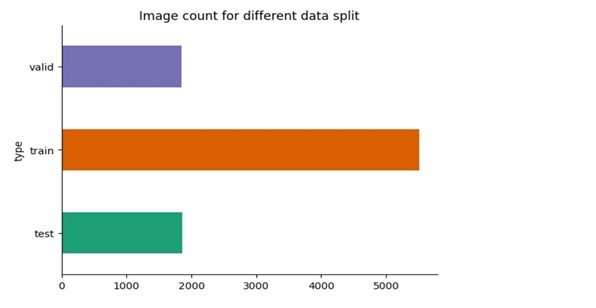
\includegraphics[scale=0.3]{figures/graph2.jpg}
    \caption{Example figure in \LaTeX.}
    \label{fig:chart_a}
\end{figure}


\subsection{Data Agumentation}
In order to increase the diversity of input data, data augmentation is used to add authentic yet unpredictable modifications to the training dataset that is supplied for neural network models. By minimally modifying the photos, it seeks to produce a copy of the original dataset. The method increases both the amount as well as the standard of the data. TensorFlow's Image Data Generator is used to apply different image-level alterations, such as height and width shifting, enlargement, and other required modifications, to the dataset. By making these little changes, the original dataset may be replicated with a greater degree of variability in the data. Rotation, width shift, zoom, and horizontal inversion are the four specific procedures that are used. The other changes are also done in this manner to make the dataset more diverse. In order to avoid underfitting and guarantee that the model gains knowledge from a variety of instances, image augmentation is especially applied to the training data.
\begin{figure}[ht]
    \centering
    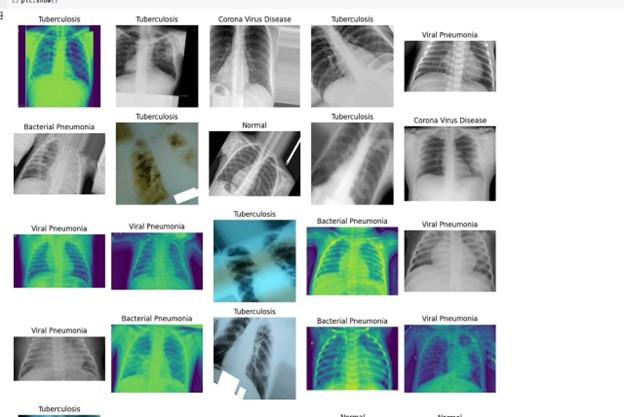
\includegraphics[scale=0.3]{figures/scan .jpg}
    \caption{Example figure in \LaTeX.}
    \label{fig:chart_a}
\end{figure}
\section {Implementation}
prediction of lung disease outbreaks is VGG 19, Mobile Net, and RestNet. When the result parameter indicates whether a lung disease epidemic is present or not, it works well for binary categorization applications. Based on input parameters such as patient statistics, surroundings, and past illness trends, the model calculates the likelihood that an epidemic will occur. VGG 19 measures how predictor variables and the chance of an outbreak of lung disease are related to each other by matching an exponential function to the input data. Model parameters help with understanding and risk evaluation by revealing the intensity and course of relationships. These models, regardless of their clarity, have several benefits, such as resilience Establishing predictive algorithms that can precisely and promptly anticipate epidemics of lung diseases is the last step. Prediction strength and accuracy are improved by combined learning techniques. Metrics for evaluating models, such as the degree of consciousness and particularity, are used to measure their predictive power and direct their modification. Model adjustment and ongoing monitoring respond to varying data distributions. By clarifying the primary variables influencing forecasted results, understanding tools promote the involvement of stakeholders and decision-making. Preventive treatments and utilization of resource techniques are made possible by incorporating public health monitoring systems and systems that support clinical decisions.

A convolutional neural network-based deep learning model is developed to identify the kind of lung illness by extracting relevant data from the input picture during training and assessment. It is possible to gain additional insight into the demand for computational resources within the healthcare industry and the potential of predictive analytics and modeling for analyzing healthcare management today and preventing global disease outbreaks in the future by addressing research challenges. The earlier pertinent preventative measures are implemented, the more quickly the disease outbreak can be prevented. To determine how well the model can detect the condition, it is evaluated using a variety of classification measures, including the f1 score and precision score. The model will be trained and predicted entirely in Python, and several libraries including Tensorflow, OpenCV, and Keras will be utilized to construct the model and store it locally for further prediction and improvement. 

A foundational statistical approach used in healthcare predictive analytics for the to input sound, speed of computation, and convenience of use.
\subsection{VGG 19}
The VGG19 Model, sometimes referred to as the "Visual Geometry Group 19-layer model," is a complex convolutional neural network (CNN) architecture that is used to integrate deep learning models for computer vision applications. It is primarily focused on picture classification problems, such as identifying objects and features in photographs. The sixteen-layer VGG16 model has been replaced by the more advanced VGG19 model. As one of the most advanced convolutional neural networks at the moment, VGG19, on the other hand, offers an improved version with 16 convolutional layers and 3 fully connected layers. Because of its complexity of 19 layers, the model is capable of representing intricate hierarchical characteristics, improving its performance in picture classification tasks. The constant implementation of max-pooling layers and 3x3 convolutional filters throughout VGG19's design makes understanding and execution easier. Significant computer vision applications, such as object detection and picture segmentation, can benefit from the contributions made by the different layers.
\begin{figure}[ht]
    \centering
    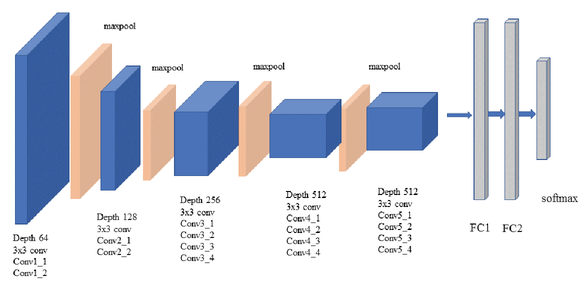
\includegraphics[scale=0.8]{figures/Picture1.png}
    \caption{Example figure in \LaTeX.}
    \label{fig:chart_a}
\end{figure}
of accuracy. The principles behind its design have an impact on the evolution of later neural network designs, therefore its contributions go beyond simple picture categorization. Because of its long-lasting influence on modern CNN designs, researchers have experimented with modifying and adapting VGG19 for a variety of computer vision problems.

In the field of healthcare predictive analysis, the VGG19 model is essential since it helps to categorize lung disorders. VGG19 offers a solid basis for accurately classifying lung diseases based on medical imaging data by utilizing its complex convolutional neural network architecture. VGG19's 19-layer architecture allows for precise differentiation between various lung disorders by skillfully capturing the intricate patterns and characteristics found in lung imaging. For predicting lung disease, the model is trained for 20 epochs.
After training the VGG 19 model, the performance is evaluated using evaluation metrics like the confusion matrix, accuracy score, and F1 score.  It can be seen that the accuracy of the model increases with every epoch and after 20 epochs, the accuracy of the model is around 0.7793. The confusion matrix is plotted in a graph which is shown below.
\begin{figure}[ht]
    \centering
    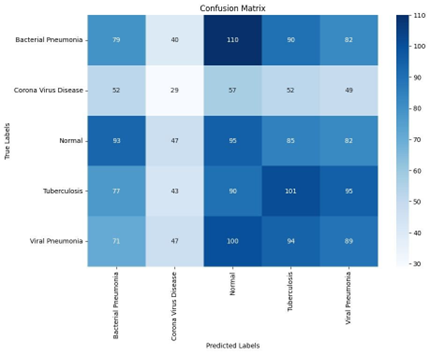
\includegraphics[scale=0.8]{figures/Picture2.png}
    \caption{Example figure in \LaTeX.}
    \label{fig:chart_a}
\end{figure}
\subsection{MobileNet}
One prominent CNN design is MobileNet, which is well-known for operating efficiently on embedded systems and mobile devices.  MobileNet, which is well-known for requiring less memory and computing power. Its main goal is to achieve high efficiency by retrieving useful information from input photos while striking a balance between precision and model size. Its effectiveness qualifies it for real-time applications on resource-constrained devices, such as smartphones and Internet of Things sensors.

The improved precision that MobileNet can achieve in tasks like object classification, segmentation using semantics, and picture classification has led to its widespread use. Building on its success, other models such as MobileNetV2 and MobileNetV3 further improve effectiveness with low computational requirements. 

It is crucial to develop models that can anticipate lung problems in advance because of function effectively on mobile and embedded devices. For mobile devices, MobileNet's insignificant memory consumption and minimal processing requirements enable the creation of accurate yet inexpensive predictive models. MobileNet enhances the effectiveness and precision of prediction tools by removing important information from medical pictures, which helps with lung disease detection and treatment promptly. MobileNet is useful for advancing healthcare technology because of its ability to strike a balance between scale and precision, particularly in the area of lung health predictive analytics.

For healthcare predictive analysis, especially for predicting lung diseases, the MobileNet architecture is trained for 20 epochs. It can be seen that the accuracy of the model varies with every epoch and after 20  epochs, the accuracy is 0.8286. Also, better accuracy is seen at the 16th epoch with 0.8388. A confusion matrix is also plotted which visually represents the performance of the model with different classes of input images.
\begin{figure}[ht]
    \centering
    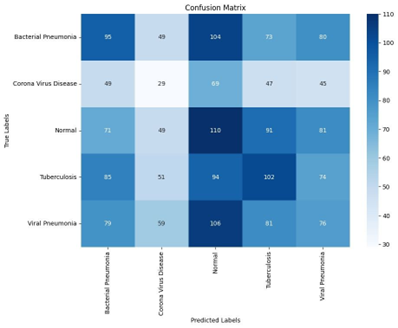
\includegraphics[scale=0.8]{figures/Picture3.png}
    \caption{Example figure in \LaTeX.}
    \label{fig:chart_a}
\end{figure}
\subsection{ResNet}
ResNet, or residual networks, is a key component of healthcare predictive analysis, especially in lung disease prediction research. Its unique architecture creates redundant connections, which enable the development of extremely complex neural networks. ResNet’s design is also ideal for transfer learning, which allows existing models to be improved on particular datasets associated with lung disease prediction. ResNet minimizes optimization and helps get over the issue of disappearing gradients that arise frequently while training deep networks. ResNet does this by employing residual learning, in which the network learns residual functions linked to the layer inputs. Because ResNet accelerates the creation of models and minimizes the requirement for huge labeled datasets, it is the method of choice for healthcare predictive analytic projects with sparse data. Doctors now have an effective tool for the early identification of conditions including TB, pneumonia, and lung cancer due to their capacity to identify minute details and anomalies in medical imaging. ResNet's deep layers improve the model in comprehending intricate relationships and patterns in medical imaging data, which increases its accuracy in forecasting when it comes to lung disorders. ResNet's adaptability to various imaging techniques, such as X-rays and computed tomography (CT), is very useful in the healthcare predictive analysis of lung disorders. 

Through the use of ResNet's features, scholars and healthcare professionals may investigate innovative methods to improve the quality of life for patients, facilitate early treatments, and possibly save lives in the fight against lung illnesses. Furthermore, in real-world healthcare conditions, where data might be complex and broad, ResNet's capacity to accommodate interference and differences in picture quality makes it valuable. For this study, the ResNet model is trained for 5 epochs and it is seen that the accuracy is not good as compared to the other models which is around 0.2196. So further training the model with the ResNet model was stopped as the accuracy was not up to the mark. 





\section{Summary}
Write a summary of this chapter.

~\\[5em]
\noindent
{\huge\textbf{Note:}} In the case of \textbf{software engineering} project a Chapter ``\textbf{Testing and Validation}'' should precede the ``Results'' chapter. See Section~\ref{subsec:se_chpters} for report organization of such project. 

